%--------------------
% Packages
% -------------------
\documentclass[11pt,a4paper,titlepage]{article}
\usepackage[utf8]{inputenc}
\usepackage[T1]{fontenc}
\usepackage{outlines}
\usepackage{booktabs}
\usepackage{mathptmx} % Use Times Font
\usepackage{subcaption}
\usepackage[toc,page]{appendix}
\usepackage[section]{placeins}
\usepackage[pdftex]{graphicx} % Required for including pictures
\usepackage[pdftex,linkcolor=black,pdfborder={0 0 0}]{hyperref} % Format links for pdf
\usepackage{calc} % To reset the counter in the document after title page
\usepackage{enumitem} % Includes lists

\frenchspacing % No double spacing between sentences
\linespread{1.2} % Set linespace
\usepackage[a4paper, lmargin=0.1666\paperwidth, rmargin=0.1666\paperwidth, tmargin=0.1111\paperheight, bmargin=0.1111\paperheight]{geometry} %margins

\usepackage[all]{nowidow} % Tries to remove widows
\usepackage[protrusion=true,expansion=true]{microtype} % Improves typography, load after fontpackage is selected
\usepackage{csquotes}
\usepackage[style=ieee,backend=bibtex]{biblatex}
\addbibresource{bibliography.bib}

%-----------------------
% Set pdf information and add title, fill in the fields
%-----------------------
\hypersetup{ 	
pdfsubject = {COM00032H},
pdftitle = {MLPG Open Assessment},
pdfauthor = {Y3843100}
}

\title{MLPG Open Assessment COM00032H}


\author{Exam No: Y3843100}

\date{\today}
%-----------------------
% Begin document
%-----------------------
\begin{document}


\maketitle


\section{Conditional independence in Bayesian networks}

\paragraph{Independent pairs}
\[\{(A,C),(A,E),(A,F),(B,C),(B,E),(B,F),(D,C),(D,E),\]
  \[(D,F),(H,A),(H,B),(H,C),(H,D),(H,E),(H,F),(H,G)\}\]

\paragraph{Independent pairs conditioned on \(Z = \{C,G\}\)}
There are no \textit{conditionally} independent pairs, yet
\[\{(H,A),(H,B),(H,D),(H,E),(H,F)\}\]
still remain unconditionally independent

\paragraph{Markov equivalent DAG}
Reverse edges but maintain immoralities, i.e. reverse \(B\) edges \textit{fig \ref{fig:1.3}}

\begin{figure}[htb]
  \centering
    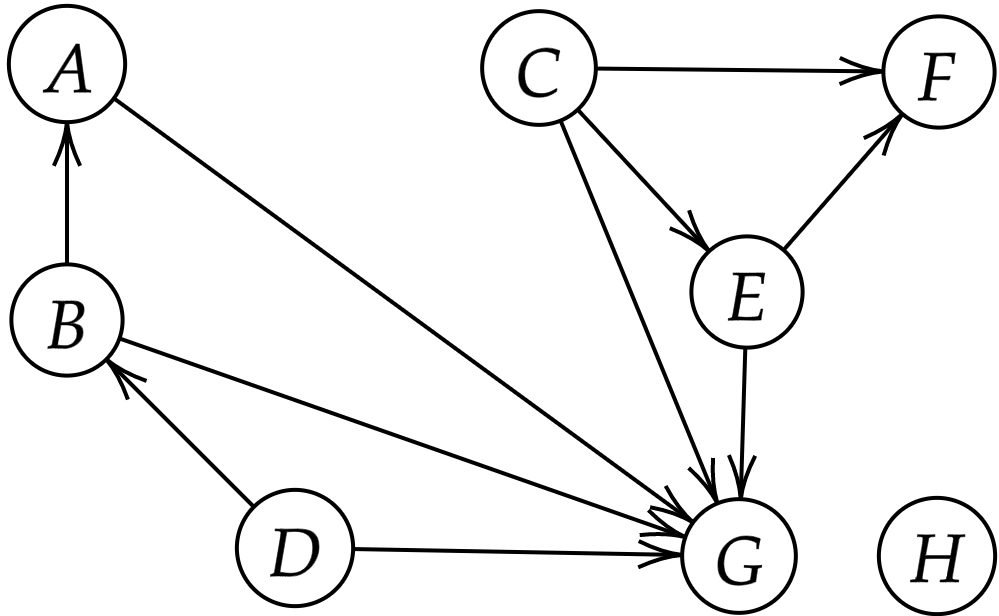
\includegraphics[width=0.5\textwidth]{../q1/fig13.png}
    \caption{Question 1.3 Markov equivalent DAG}
  \label{fig:1.3}
\end{figure}

\paragraph{Non-Markov equivalent DAG}
Change immoralities, i.e. reverse all edges from \(G\) \textit{fig \ref{fig:1.4}}
\begin{figure}[htb]
  \centering
    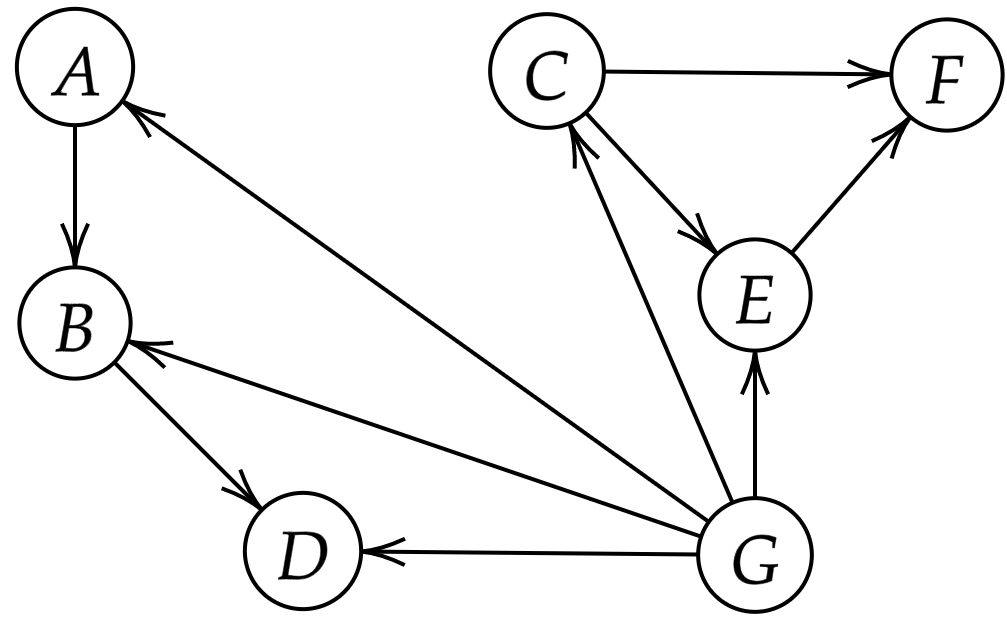
\includegraphics[width=0.5\textwidth]{../q1/fig14.png}
    \caption{Question 1.4 Non-Markov equivalent DAG}
  \label{fig:1.4}
\end{figure}

\section{House prices with STAN}
%TODO: Offload all data manipulation in the .py files and not in the q2data
%TODO: Make sure all files embedded the model as a str
  \subsection{A simple model (figs \ref{fig:2.1} and \ref{tab:2.1})}
  The first step in checking if our posterior is in the right direction is assessing if the MCMC has converged. This is the case for this model as \(\hat{R} = 1\), which is also observed by the beta plots. Furthermore the 95\% confidence interval is reasonably tight around the mean, indicating they are good posterior predictions.
  The preference for MCMC sampling over variational inference was due to the fact that the size of our dataset and the length of this assessment permits the usage of the more computationally intensive method. In addition, the asymptotic correctness of the posterior justifies the larger computational expense \parencite{BleiVI}. Empirical tests show that the STAN default of 1000 iterations (2000 samples) and 4 chains is enough for convergence.
  %This model asserts the assumption that althought the data represents the house prices of two distinct locations, the price formation given Age and Size is the same for the two regions.

  \subsection{A less simple model (figs. \ref{fig:2.2} and \ref{tab:2.2})}
  Denoting that size has a positive effect on price does not affect performance. This is potentially due to the fact that the data already embodies this fact and explicitly stating it does not give us any new knowledge.

  \subsection{Two models (figs. \ref{fig:2.3_0},\ref{fig:2.3_1})}
  %TODO: Discuss the intercept values being so different
  Houses in 0 get cheaper with age, which was obfuscated in 2.2. Splitting also reduces noise. The higher certainty in our split models is also reflected by the superior \texttt{lp\_\_}.

  \subsection{A compromise model (figs. \ref{tab:2.4}, \ref{fig:2.4} \ref{fig:2.4_bnet})}
  We create a hierarchical model \parencite{MultilevelHM} that has variant slopes, but maintains the intercept across locales \(y_i = \alpha + \beta_{j[i]} x_i + \epsilon_i \) with all \(\epsilon \sim N(0,\sigma^{2})\) \parencite{VaryingAlpha}. With it we are able to capture the Age difference and still share some global knowledge via the intercept.

\section{VI vs MCMC}
\paragraph{}
HMC posterior approximations start with a random set of parameters \(\theta\) which are updated over a number of iterations according to a randomly sampled momentum vector \(\rho\). The update follows a Hamiltonian process where \(H(\rho,\theta) = -\log p(\rho \mid \theta) - \log p(\theta)\). The new state \((\rho^*,\theta^*)\) is evaluated against a Metropolis acceptance test \(min(1, \exp(H(\rho,\theta)-H(\rho^*,\theta^*)))\). If not accepted, the previous \(\theta\) is recovered and a new random sample is drawn for the next iteration \parencite{betancourt2015hamiltonian}.
\paragraph{}
STAN's VI approximates posteriors by using automatic differentiation (AD) to transform the variables into a co-ordinate space where it asserts that the new transformed density is Gaussian. Then it uses the transformed support to maximise the evidence lower bound (ELBO, which is in essence the analytical form of KL divergence between our approximation and the true distribution) \parencite{ADVISTAN}. The maximisation is done via gradient ascend.
\paragraph{}
VI is faster and can be used on large datasets but specifically for STAN if a Gaussian mixture model is not appropriate for our problem, VI will struggle. MCMC is asymptotically precise yet is computationally intensive and multimodal distributions can confuse it.

\section{Hidden Markov models}
%TODO: explain forward and backward prob in EM
Forward \(\alpha(h_t)\) and backward \(\beta(h_t)\) probabilities are useful when doing the M (and the respectively the obfuscated E) steps when calculating the transition probabilities \(p^{new}(h_{t+1} = i^\prime \mid h_t = i)\) by computing the hidden state marginals \(p(h_t \mid v_{1:T}) = \frac{\alpha(h_t)\beta(h_t)}{\sum_{h^{\prime}_t}\alpha(h_t^\prime)\beta(h_t^\prime)}\) and for the emission probabilities \(p^{new}(v_t = j \mid h_t = i)\) the pairwise marginals \(p(h_t, h_{t+1} \mid v_{1:T}) \propto \alpha(h_t)p(v_{t_1} \mid h_{t+1})p(h_{t+1} \mid h_t)\beta(h_t)\).

\begin{appendices}
  \section{Tables and Plots}
    \begin{figure}[htb]
      \centering
        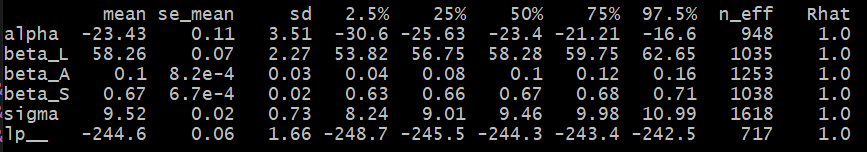
\includegraphics[width=\textwidth]{../q21/q21_summary_table.png}
        \caption{Question 2.1 posterior table summary}
      \label{tab:2.1}
    \end{figure}

    \begin{figure}[htb]
      \centering
        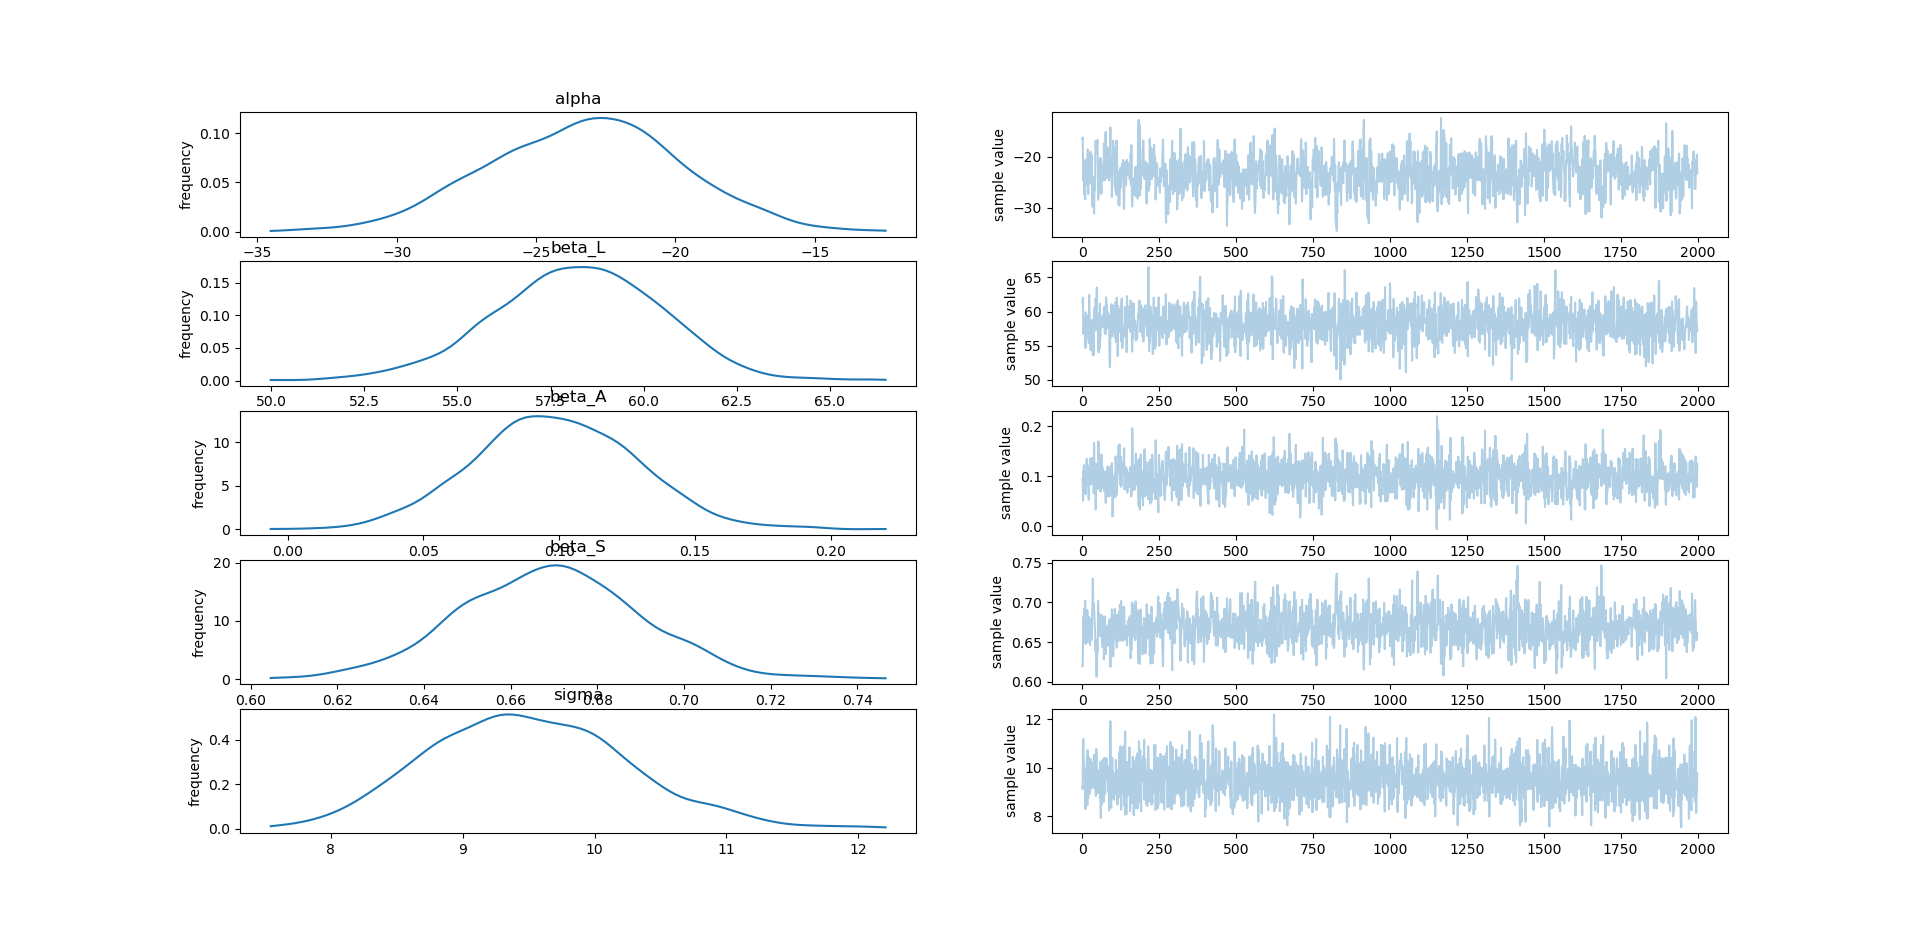
\includegraphics[width=\textwidth]{../q21/separated_features.png}
        \caption{Question 2.1 plot summary}
      \label{fig:2.1}
    \end{figure}

    \begin{figure}[htb]
      \centering
        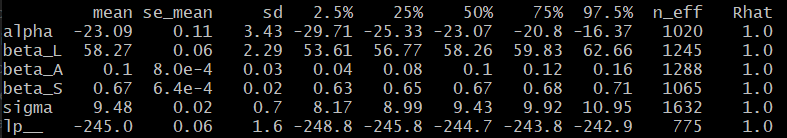
\includegraphics[width=\textwidth]{../q22/q22_table_summary.png}
        \caption{Question 2.2 posterior table summary}
      \label{tab:2.2}
    \end{figure}

    \begin{figure}[htb]
      \centering
        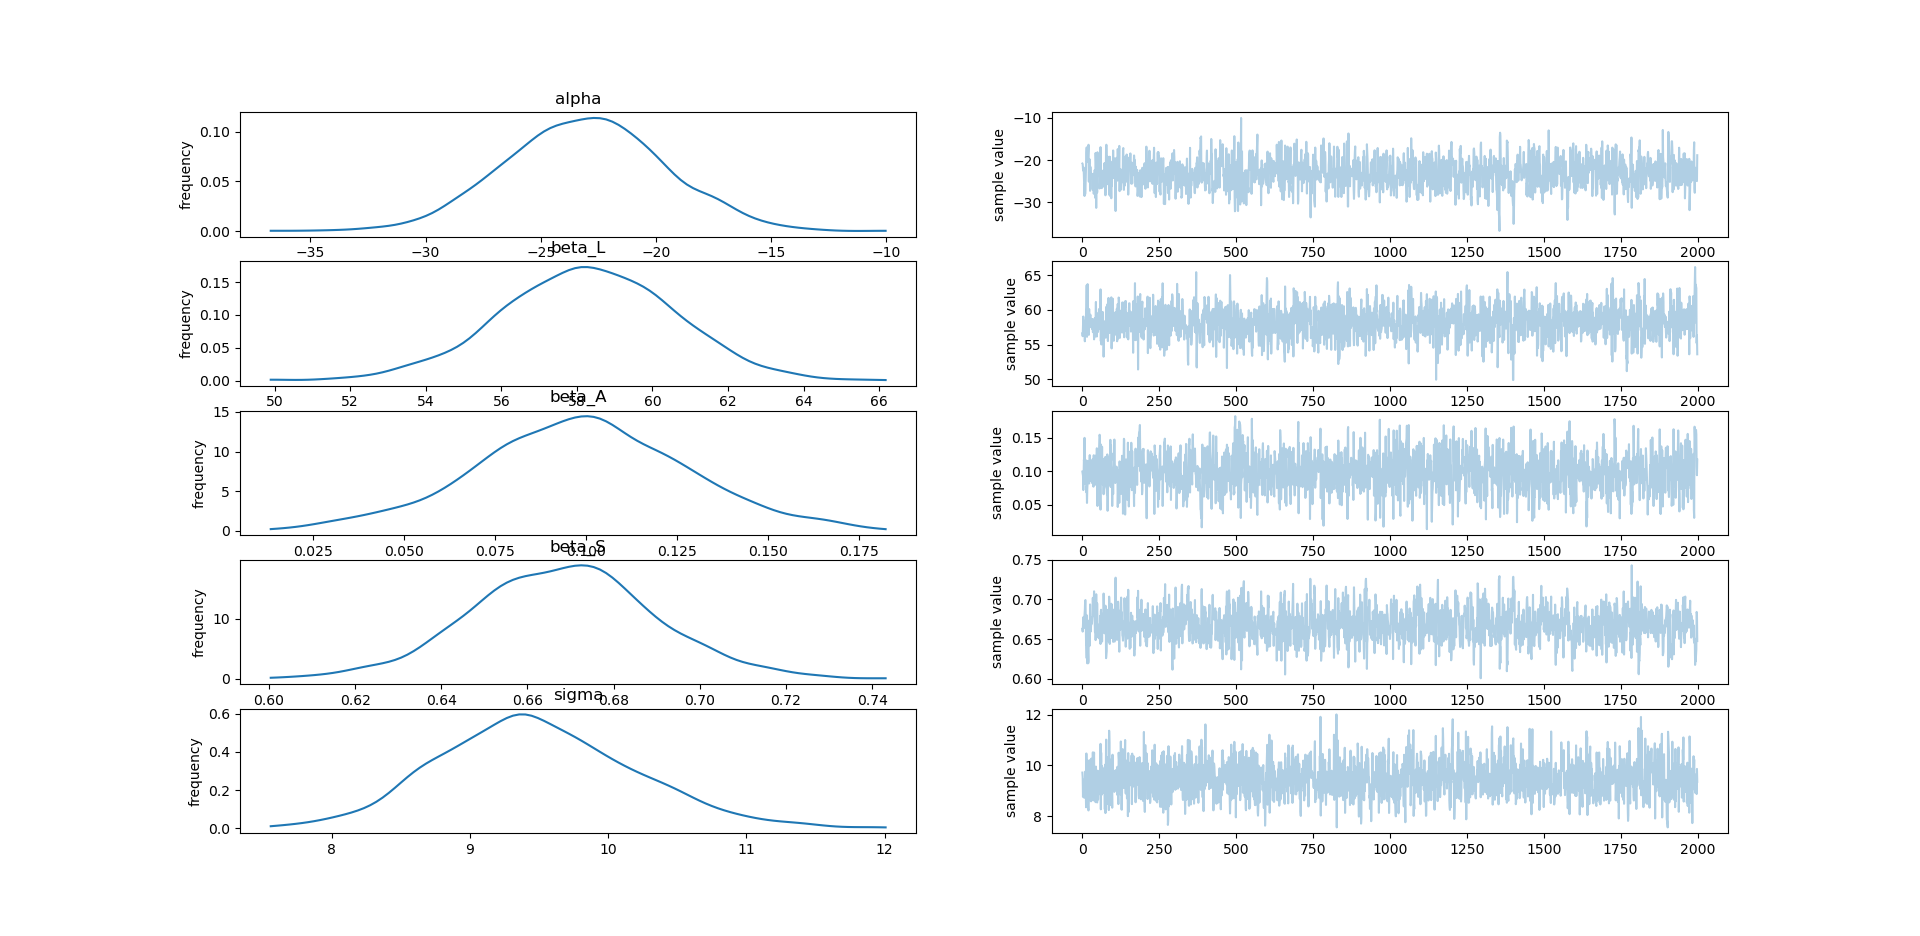
\includegraphics[width=\textwidth]{../q22/q22_plot_summary.png}
        \caption{Question 2.2 plot summary}
      \label{fig:2.2}
    \end{figure}

    \begin{figure}[htb]
      \centering
      \begin{subfigure}[b]{\textwidth}
        \centering
        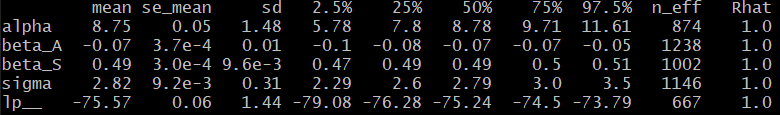
\includegraphics[width=\textwidth]{../q23/q23_table_summary_L0.png}
        \caption{posterior table summary}
      \end{subfigure}
      \hfill
      \begin{subfigure}[b]{\textwidth}
        \centering
        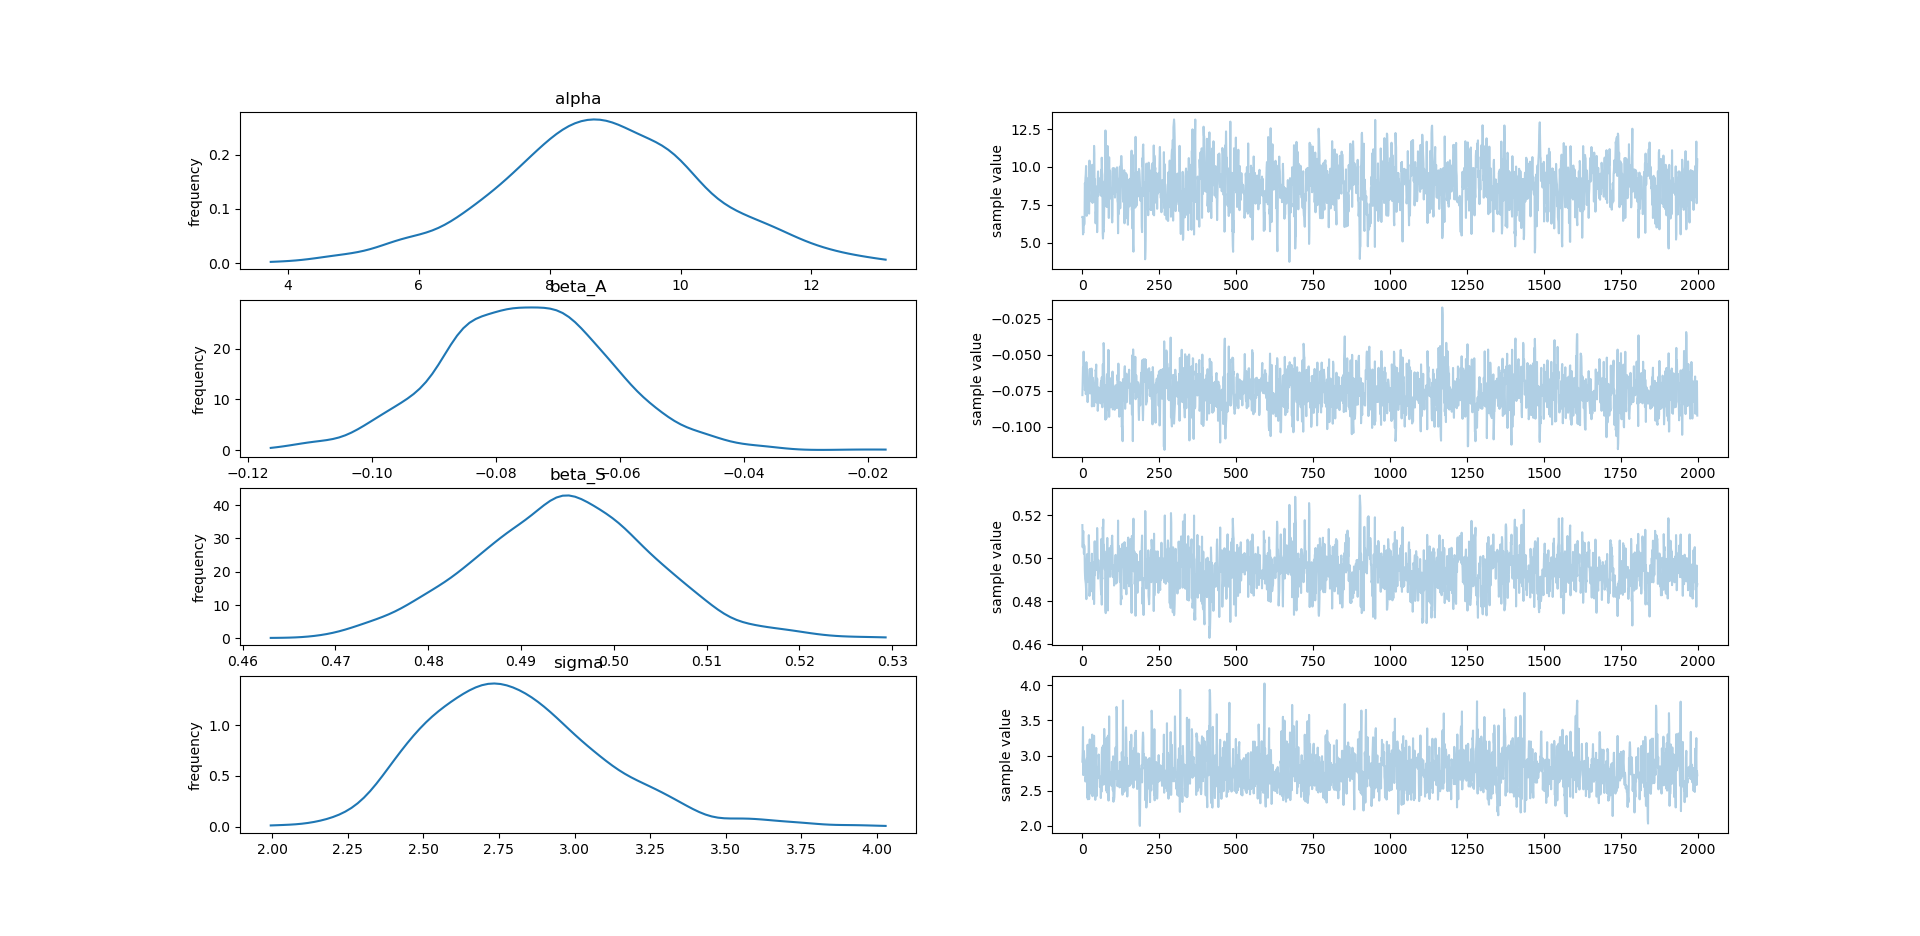
\includegraphics[width=\textwidth]{../q23/q23_plot_summary_L0.png}
        \caption{plot summary}
      \end{subfigure}
      \caption{Question 2.3 Locale 0}
      \label{fig:2.3_0}
    \end{figure}

    \begin{figure}[htb]
      \centering
      \begin{subfigure}[b]{\textwidth}
        \centering
        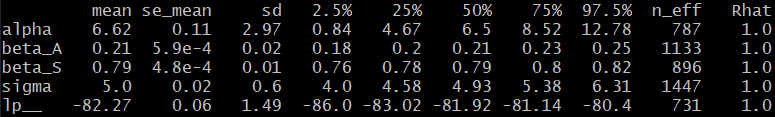
\includegraphics[width=\textwidth]{../q23/q23_table_summary_L1.png}
        \caption{posterior table summary}
      \end{subfigure}
      \hfill
      \begin{subfigure}[b]{\textwidth}
        \centering
        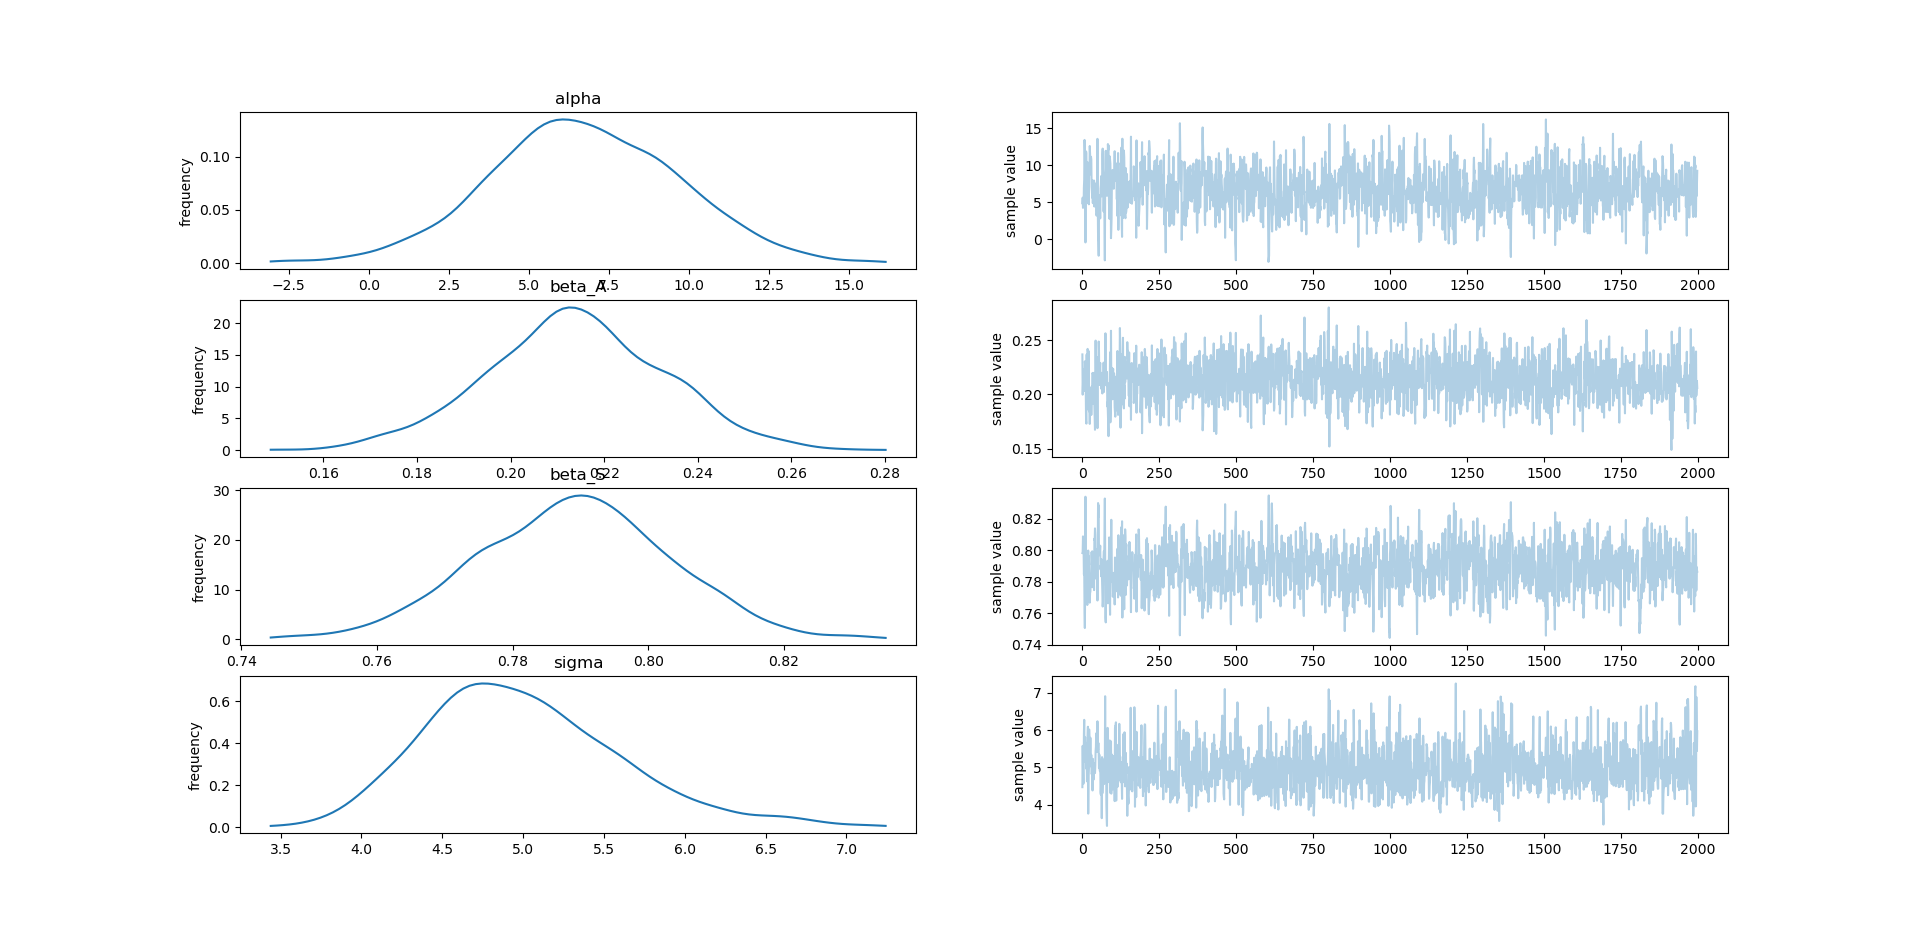
\includegraphics[width=\textwidth]{../q23/q23_plot_summary_L1.png}
        \caption{plot summary}
      \end{subfigure}
      \caption{Question 2.3 Locale 1}
      \label{fig:2.3_1}
    \end{figure}

    \begin{figure}[htb]
      \centering
        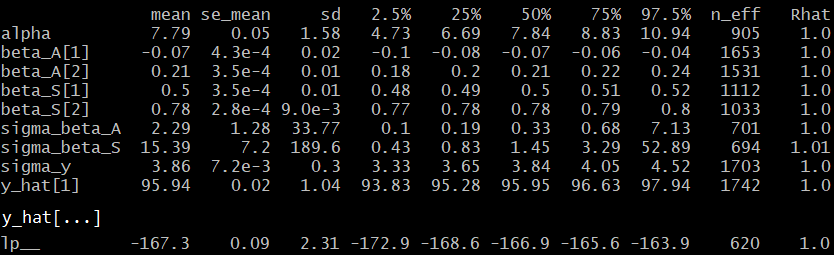
\includegraphics[width=0.95\textwidth]{../q24/q24_table_summary.png}
        \caption{Question 2.4 posterior table summary}
      \label{tab:2.4}
    \end{figure}

    \begin{figure}[htb]
      \centering
        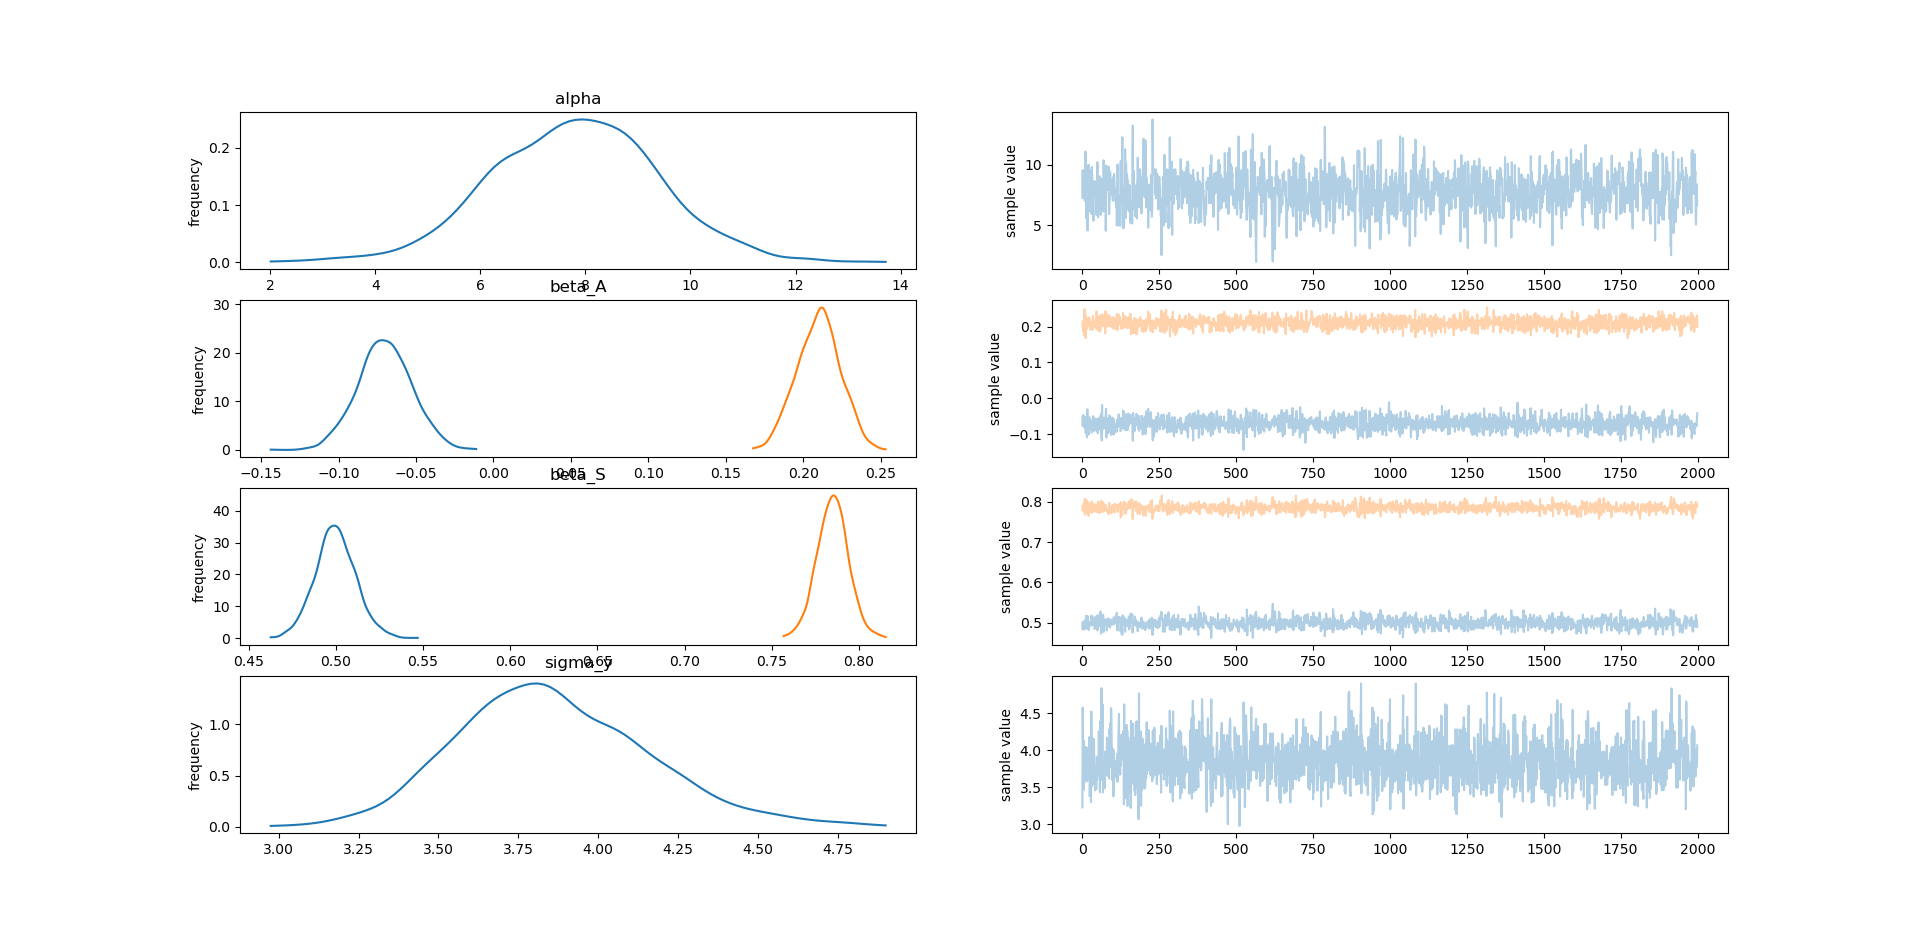
\includegraphics[width=\textwidth]{../q24/q24_plot_summary.png}
        \caption{Question 2.4 plot summary}
      \label{fig:2.4}
    \end{figure}

    \begin{figure}[htb]
      \centering
        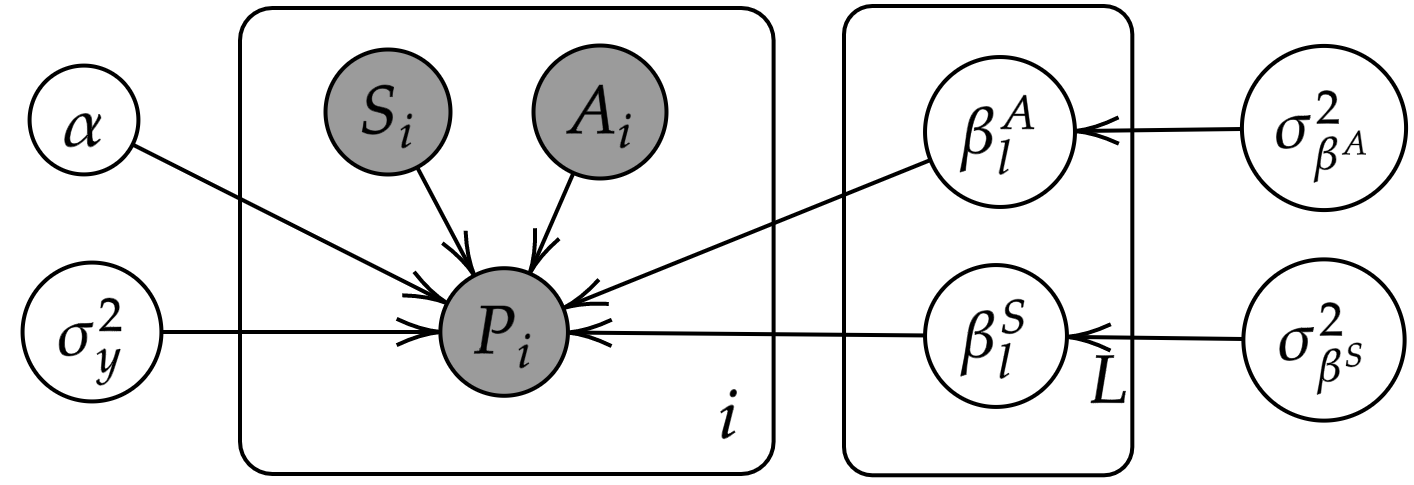
\includegraphics[width=\textwidth]{../q24/q24_bnet.png}
        \caption{Question 2.4 model as Bayesian network}
      \label{fig:2.4_bnet}
    \end{figure}
\end{appendices}

\printbibliography
\end{document}